\documentclass[12pt,a4paper,leqno]{report}

\usepackage[T1]{fontenc}
\usepackage[english]{babel}
\usepackage{amsthm}
\usepackage{amsfonts}
\usepackage{amsmath}
\usepackage{amssymb}
\usepackage{tikz}
\usepackage{listings}

\newcommand{\R}{\mathbb{R}}
\newcommand{\C}{\mathbb{C}}
\newcommand{\Q}{\mathbb{Q}}
\newcommand{\N}{\mathbb{N}}
\newcommand{\No}{\mathbb{N}_0}
\newcommand{\Z}{\mathbb{Z}}
\newcommand{\diam}{\operatorname{diam}}

\theoremstyle{plain}
\newtheorem{equa}[equation]{Equation}
\newtheorem{lem}[equation]{Lemma}
\newtheorem{prop}[equation]{Proposition}
\newtheorem{cor}[equation]{Corollary}

\theoremstyle{definition}
\newtheorem{defi}[equation]{definition}
\newtheorem{conj}[equation]{Conjecture}
\newtheorem{example}[equation]{Example}
\theoremstyle{remark}
\newtheorem{note}[equation]{Note}

\pagestyle{plain}
\makeatletter
\renewcommand{\@seccntformat}[1]{}
\makeatother
\setcounter{page}{1}
\addtolength{\hoffset}{-1.15cm}
\addtolength{\textwidth}{2.3cm}
\addtolength{\voffset}{0.45cm}
\addtolength{\textheight}{-0.9cm}

\graphicspath{ {../figures/} }

\title{Data Analytics 2 - Market Basket Analysis}
\author{Tuomo Kareoja}
\date{}

\begin{document}

\maketitle

\begin{table}[h!]
  \begin{center}
    \begin{tabular}{l|c|r}
      \textbf{Version Number} & \textbf{Changes} & \textbf{Date} \\
      \hline
      0.5 & Basic structure, some text and plots & 16.09.2019\\
      1.0 & Finished text and plots & 17.09.2019\\
    \end{tabular}
  \end{center}
\end{table}

\newpage

\section{Main Takeaways}


\begin{enumerate}
    
    \item Although in most product categories Blackwell and Electronidex fit together nicely by offering products in different categories or
    product in different price ranges, with PC:s, Displays and Tablets there is considerable overlap. This is worrying as these 3
    categories create 45 \% of Blackwells' profits.

    \item Electronidex has a huge portfolio of over 4000 products and as there are only slightly over 10000
    transactions with more than 1 unique product, it is hard to find reliable connections for
    buying certain products together.

    \item If we add the product brand to the analysis, the results are still weak. The one interesting
    thing in this level is the way that apple products are often bought together with other
    apple products. Apple is also the most popular brand in transactions, being over 2 times
    more common than the next one which OWC (who make Apple accessories).

    \item If we perform the market basket analysis at level of product categories, we find interesting
    connections between buying smartwatches, cameras and products of category other (these include
    a number of different products e.g. lamps with usb ports for charging other devices, connected
    thermostats etc.) and buying products belonging to the most profitable categories
    in Blackwells' product lineup: displays, tablets, pc:s, laptops, smartphones, printers and software.
    These associations offer strong cross selling possibilities as Blackwell does not itself
    offer any products in the predictive categories. Unfortunately these rules cover only
    2.7 \% of the multi-item transactions and only 0.6 \% of all transactions. This means that
    although these rules are can find a subset of transactions for cross sales, these transactions
    are quite niche and their total monetary value is questionable
    
    \item For better analysis of we would want to have information about the individual profitability
    of different items in Electronidex product lineup
 
\end{enumerate}

\section{Blackwell Product Line Comparison to Electronidex Product Line}

Blackwells' two most profitable product categories are displays and game consoles. These two groups
create 55 \% of Blackwells' profits at the moment. After these two groups
there are 6 product groups that also contribute substantially, but that are not individually on the same
level of importance as the two biggest categories. These products create 41 \% of our profits.
Below is a breakdown of our profits by percentage by product category. Extended warranties are not included
in this plot as the data that we have from them is suspicious as it seems to have copy pasted values
between different warranties.

\bigskip
{
    \centering
    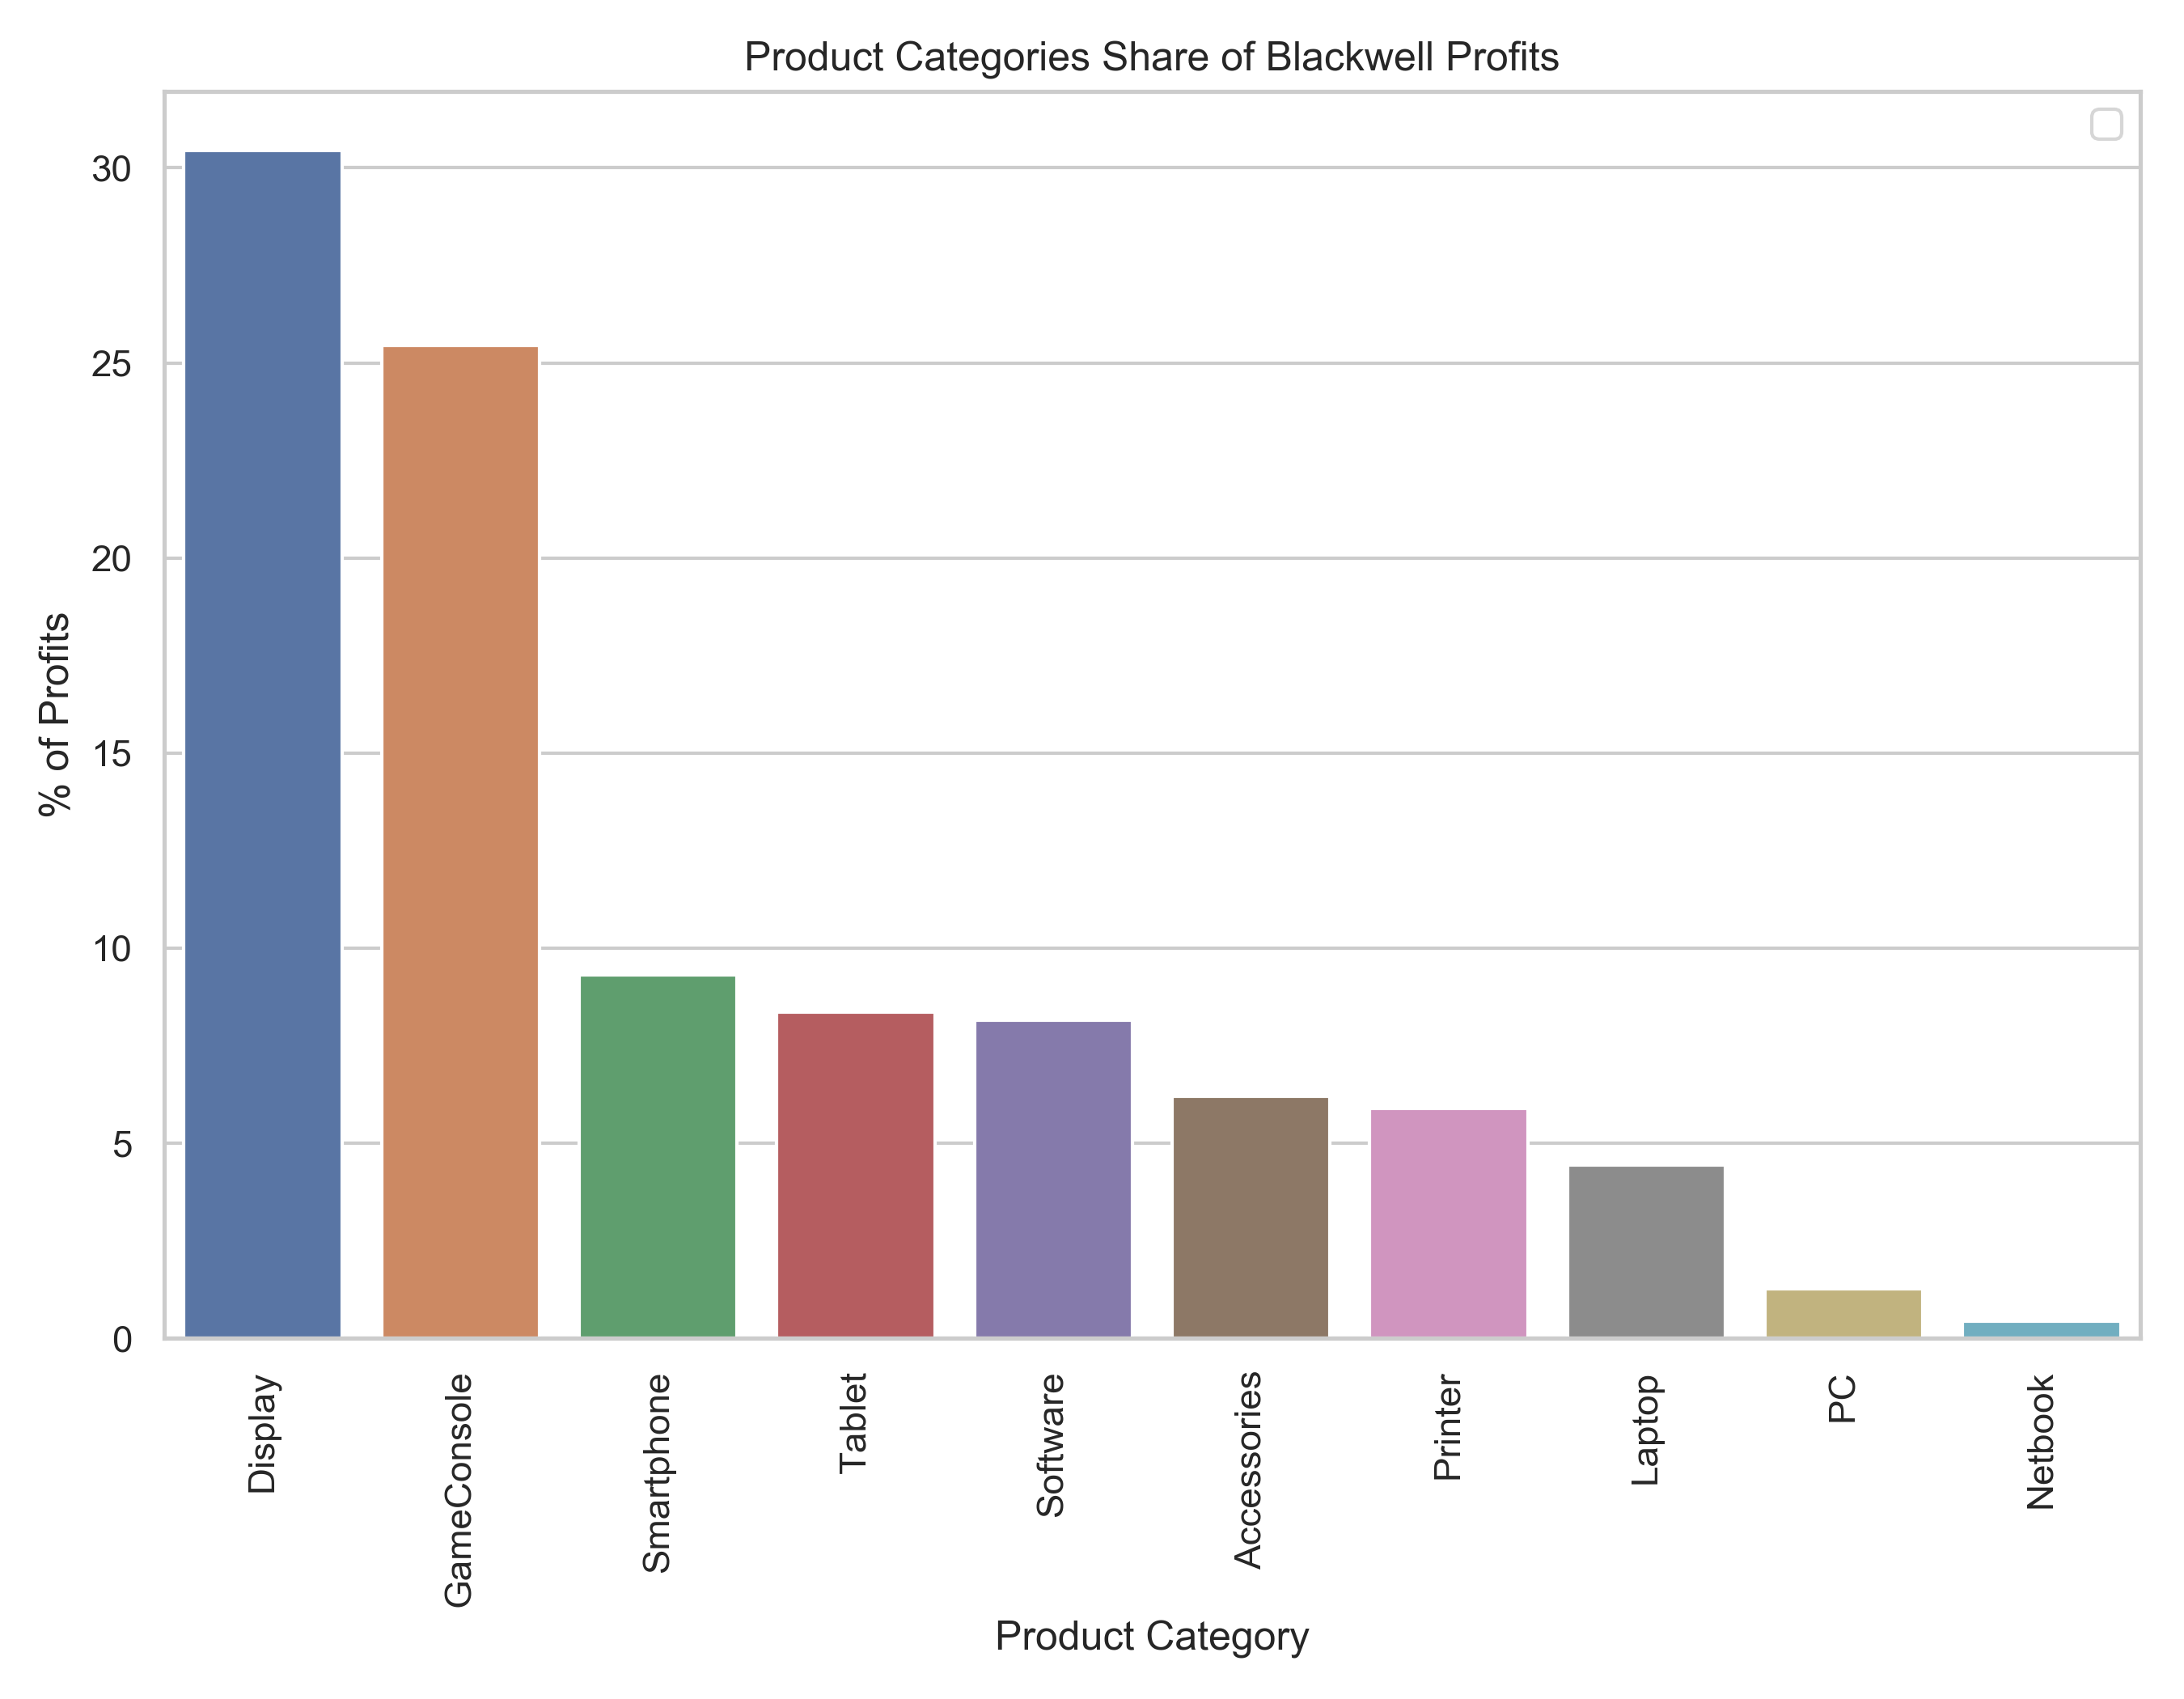
\includegraphics[width=\textwidth,height=\textheight,keepaspectratio]{blackwell_profits_share_by_product_category.png}
    \par
}
\bigskip

Next we look at the profits created from individual sales of our products. Below are plotted are our available
products sorted to product categories with their profit created per sold unit on the y-axis.
We see that our profits per product are actually quite consistent except for accessories
and one very high profit product in PC:s and another in Displays.
By comparing these to the breakdown of our profits per category we can come to the conclusion that to diversify
our profit making increasing our sales of PC:s, laptops, software, printers, tablets and smartphones would be
advisable. Especially PC:s, Laptops and Tablets offer big profits per sold product. We keep this in mind
when looking at what Electronidex has in their product lineup.

\bigskip
{
    \centering
    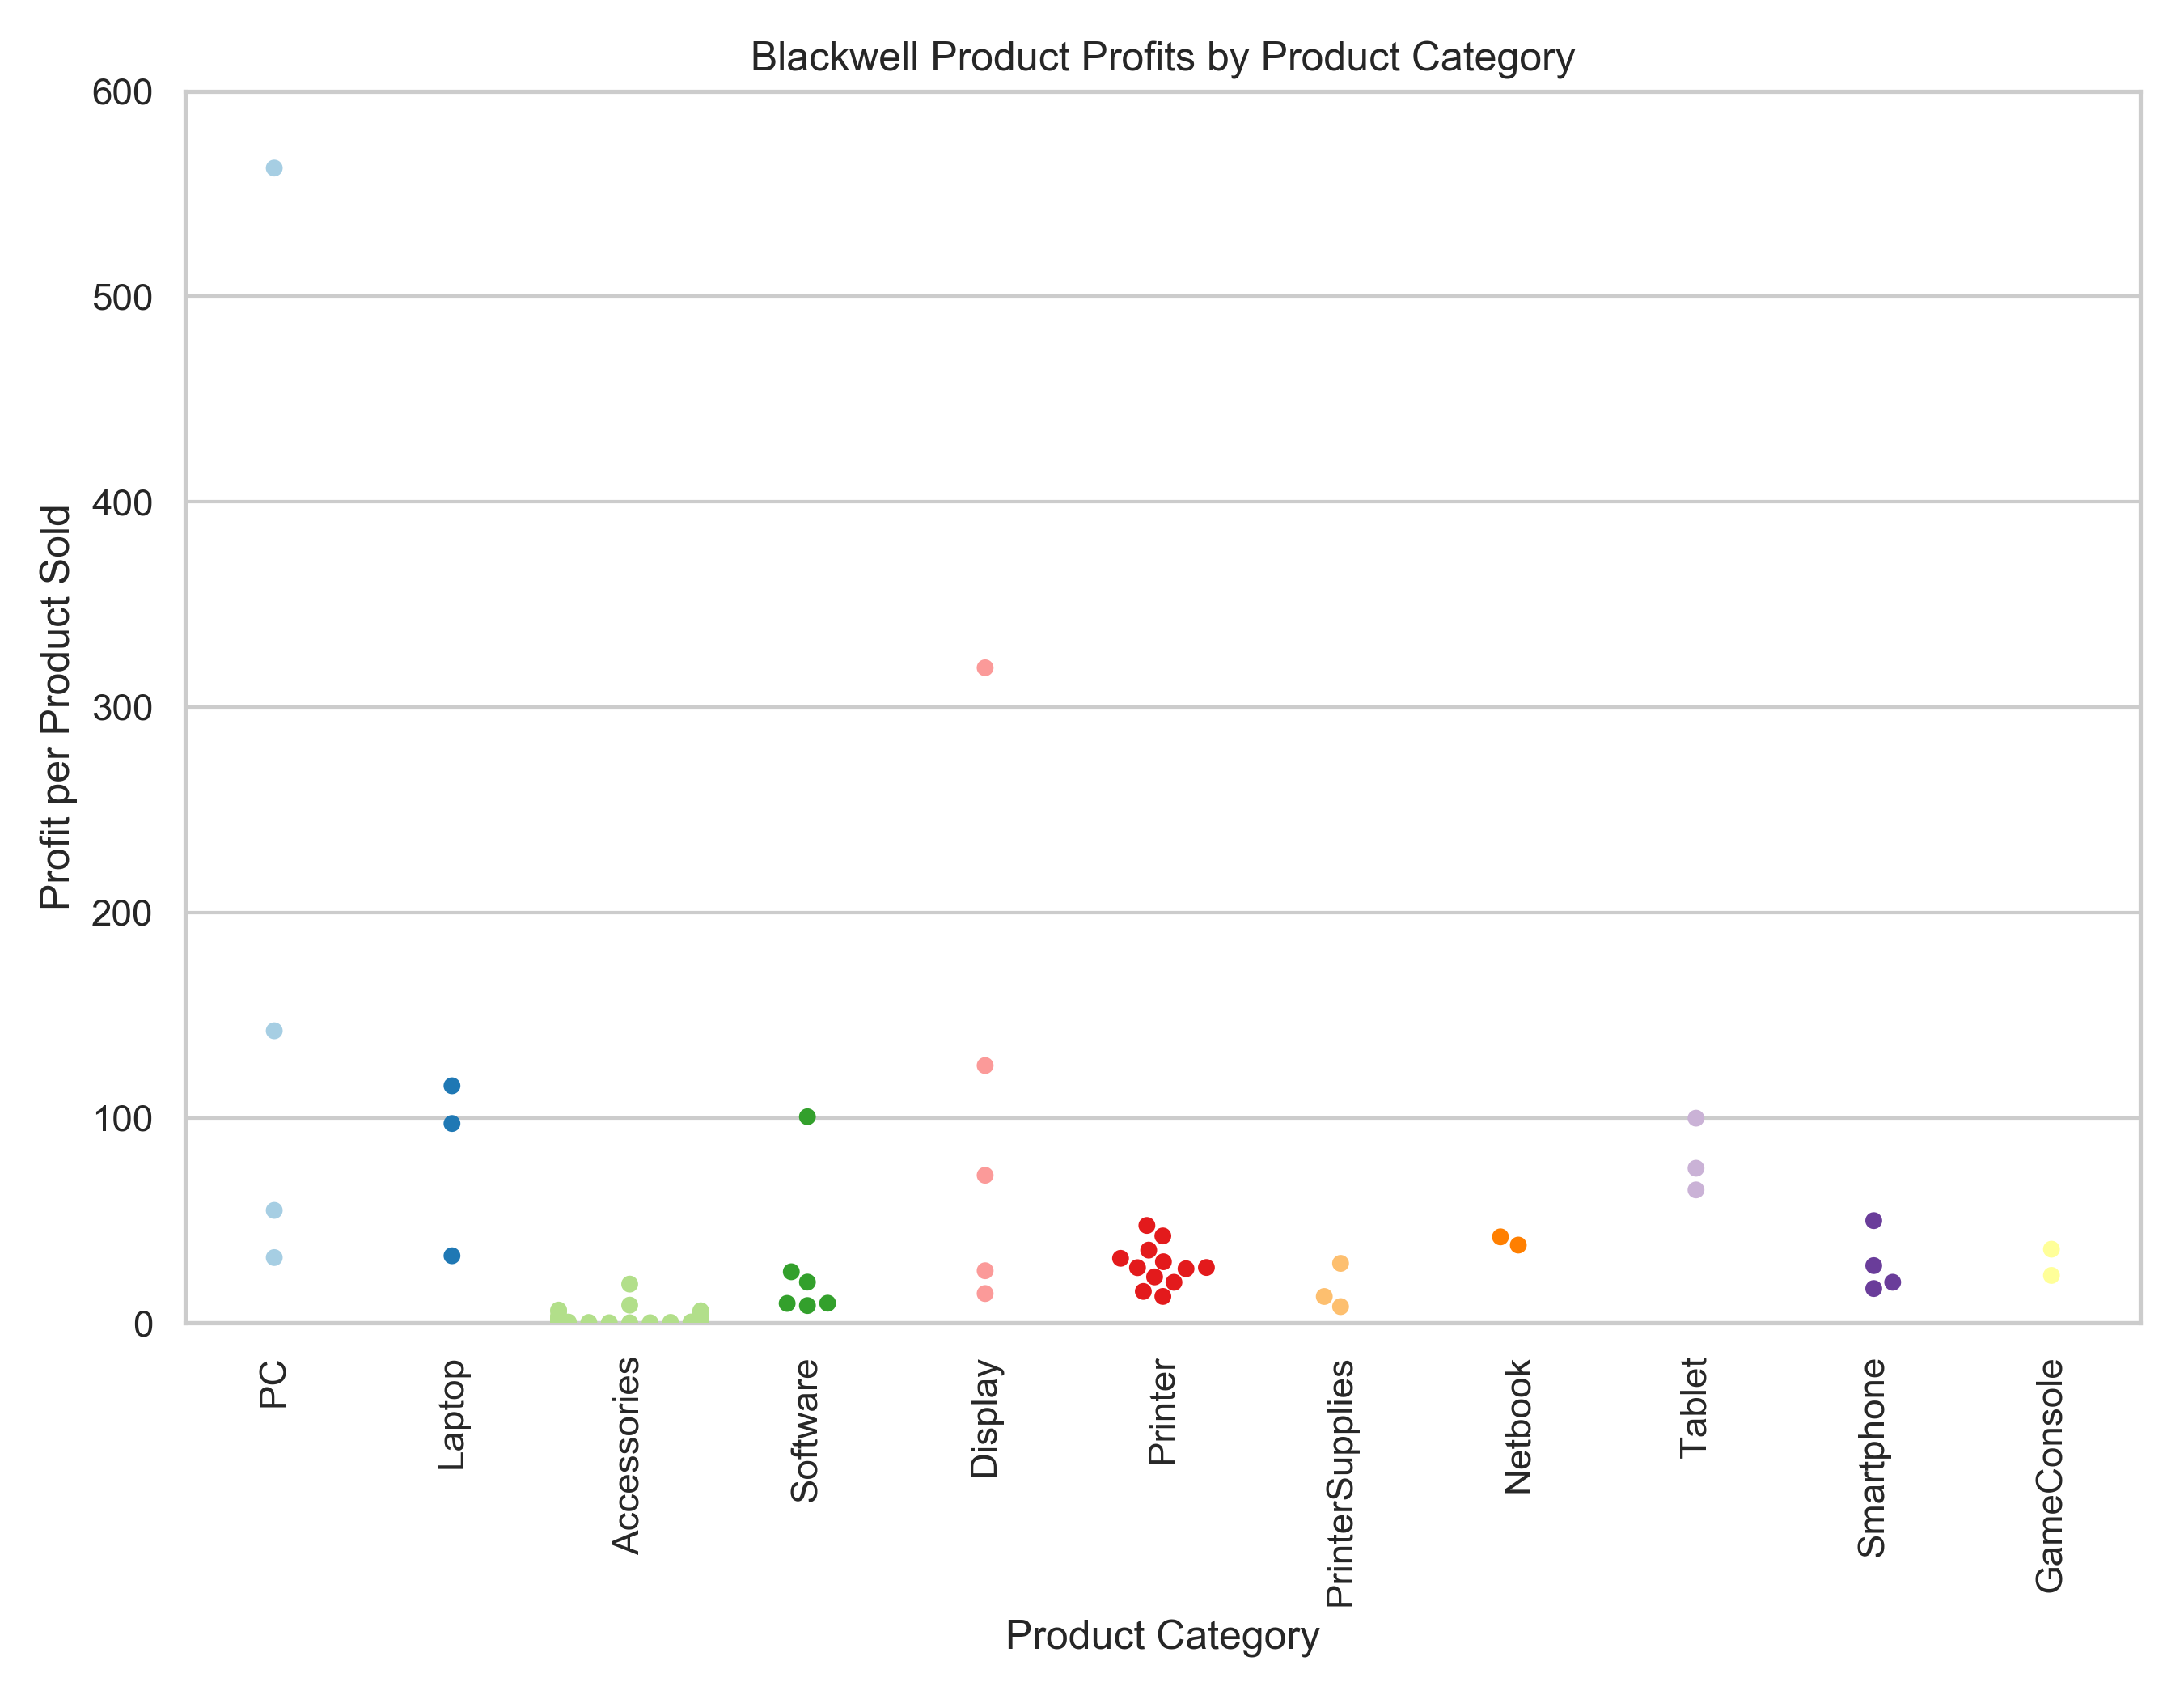
\includegraphics[width=\textwidth,height=\textheight,keepaspectratio]{blackwell_product_profitability_distribution_by_category.png}
    \par
}
\bigskip

Next we see how our product lineup matches that of Electronidex. Below is a plot Blackwells' and Electronidex
product by product categories with their list prices (in Electronindex case we used the median price of sold items
to take into account how often there are discounts or other variation that might skew the real price away from list price).
Accessories have be left out this picture as there are too many products to visualize properly. Suffice to say
that in this category there is considerable overlap if we look at just the price and category, but
accessories is a difficult category as often these are related to just certain products and in these cases
if our products are not exactly the same there will no overlap. Because of this reason we have left
accessories out from the following analysis.

\bigskip
{
    \centering
    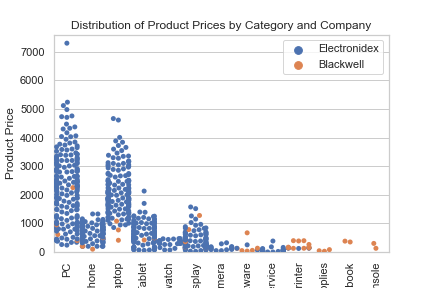
\includegraphics[width=\textwidth,height=\textheight,keepaspectratio]{product_prices_distribution_by_category_and_company.png}
    \par
}
\bigskip

We see that Electronidex has a very large product lineup that dwarfs ours.
Going trough each category we can divide the categories into ones that have little or no overlap, ones that have overlap,
but our products are differentiated by price, and ones where there is considerable overlap:

\begin{description}
   \item [No overlap:] smartwatch, camera, software, service, printer, printer supplies, netbook, game console
   \item [Overlap, but different prices:] smartphone, laptop
   \item [Overlap, no price difference:] PC, tablet, display
\end{description}

The categories that don't overlap and that have don't have any offerings from Blackwell include smartwatches, cameras
and services. These are product categories that would just extend our lineup if we acquired Electronidex.
The product categories that we have offering and Electronidex has none or only few include software, printers,
printer supplies, netbooks and game consoles. These product categories would not need to compete with Electronidex
offering and could benefit from cross-sales. These categories make up 40 \% of our current profits.

The categories that have overlap, but where there is a price differentiation include smartphones and laptops.
In both of these categories our product add more options to the lower price range of these products. With laptops
our priciest model has similarly priced offerings from Electronidex product range but our two lower end products
would form a new low end offering to the combined product range. This is true somewhat also with smartphones
where are our cheapest phone is cheaper than any offering from Electronidex, but our other offerings
would be less clearly differentiated. Not including our highest end phone, this could still be ok, as the
low end offerings from Electronidex are more limited than the midrange offerings and our products would change this.
These two categories constitute 13 \% of our profits.

The categories where there is substantial overlap are PC:s, tablets and displays. Here our products
don't differentiate themselves from Electronidex offering by price. This means that our products
would possibly compete for the same customers. These categories form 40 \% of our current profits.

conclusions

\section{Market Basket Analysis of Electronidex Transactions}

\subsection{Product Level}

This does not work

\subsection{Brand Level}

\bigskip
{
    \centering
    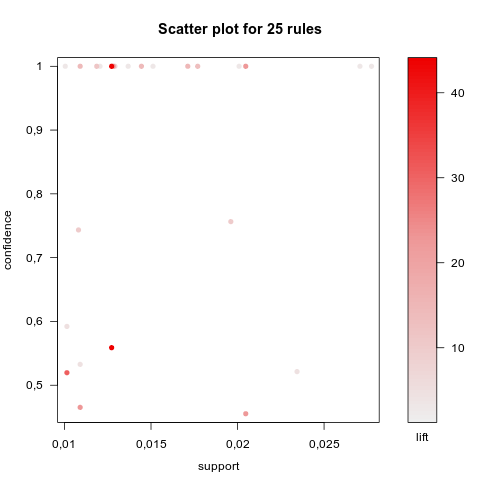
\includegraphics[width=\textwidth,height=\textheight,keepaspectratio]{apriori_brand_level_plot.png}
    \par
}
\bigskip

\bigskip
{
    \centering
    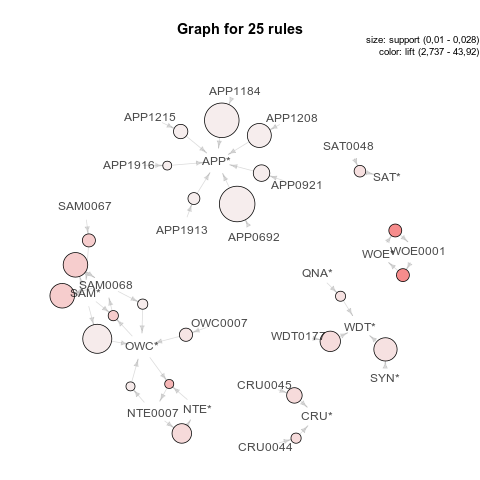
\includegraphics[width=\textwidth,height=\textheight,keepaspectratio]{apriori_brand_level_graph.png}
    \par
}
\bigskip


\subsection{Product Category Level}

\bigskip
{
    \centering
    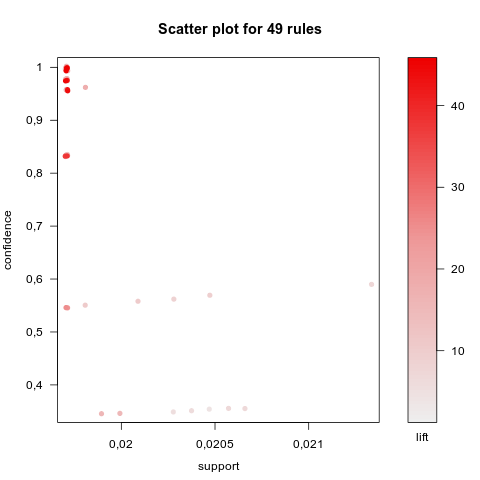
\includegraphics[width=\textwidth,height=\textheight,keepaspectratio]{apriori_product_category_level_plot.png}
    \par
}
\bigskip

\bigskip
{
    \centering
    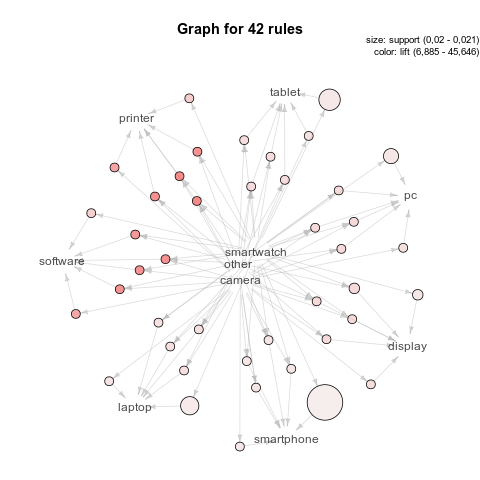
\includegraphics[width=\textwidth,height=\textheight,keepaspectratio]{apriori_product_category_level_graph.png}
    \par
}
\bigskip

\section{Suggested Next Steps}

Some text

\end{document}
